\chapter{Extracción de normales a la superficie de una nube usando PCL}

\section{Introducción}
Se ha justificado en el capítulo anterior que será el algoritmo de extracción de vectores normales el que se llevará a hardware digital para ser optimizado. 

En este capítulo, se va a estudiar en profundidad dicho algoritmo exclusivamente en el ámbito de la librería PCL ya que ésta se sirve de librerías externas como son principalmente Eigen y boost. Este estudio es necesario para comprender cómo funciona el algoritmo y así poder realizar la optimización del hardware digital obtenido a partir de éste.

Por lo tanto, se explicará tanto en alto como en bajo nivel cómo PCL estima normales a la superficie de una nube de puntos de un modo semejante al que se ha utilizado para explicar fragmentos de código en capítulos anteriores. Finalmente, se mostrará el código en C++ que será modificado y sintetizado en hardware en el siguiente capítulo.


\section{Técnica de estimación de vectores normales}

%http://mediatum.ub.tum.de/doc/800632/941254.pdf


Las normales a una superficie son una de sus características geométricas más importantes no solamente en lo que concierne a la estimación de keypoints sino a otras áreas de computación gráfica como puede ser determinar las fuentes de luz adecuadas para generar sombras y brillos u otros efectos visuales semejantes. Por esta razón, la estimación de normales es una importante característica de la librería PCL.

Si se considera una superficie, normalmente es trivial estimar la dirección de la normal en un determinado punto como el vector perpendicular a la superficie en el mismo. Sin embargo, puesto que las nubes de puntos adquiridas por los sensores son un conjunto de puntos que representan una superficie, hay dos formas de proceder para estimar normales:

\begin{itemize}
\item[•]Reconstruir la superficie que representan los puntos utilizando técnicas de reconstrucción de superficies y entonces calcular los vectores a partir de la superficie reconstruida.
\item[•]Utilizar aproximaciones para estimar las normales directamente a partir de la nube de puntos.
\end{itemize}

Dada la complejidad que implica la primera opción, se va a proceder de ahora en adelante con la segunda, estimar vectores normales a partir de puntos que representan una superficie.

El problema de determinar un vector normal a una superficie en un punto de la misma se puede aproximar mediante una de las formas más simples y claras que se pueden plantear. Esto implica la estimación de la normal a un plano tangente a la superficie en el punto estudiado junto a $k$ puntos vecinos, siendo entonces $P^k$ el mencionado conjunto y un punto en particular $p_{i} \in P^{k}$ representado por sus coordenadas mediante $p_{i}=\left\lbrace p_{i_x},p_{i_y},p_{i_z} \right\rbrace$.

El plano utilizado para aproximar la normal en un punto de la nube es representado por un punto $x$ y un vector normal $\vec{n}$ de modo que la distancia de un punto $p_{i} \in P^{k}$ al plano queda definida como:

$$d_i=(p_{i}-x)\vec{n}$$

Además, $x$ se define como el centroide de $P^{k}$ de la siguiente manera:

$$x=\frac{1}{k}\sum_{i=1}^{k} p_i$$

Considerando lo anterior, se toman valores de $x$ y $\vec{n}$ de forma que, resolviendo un problema de mínimos cuadrados, $d_i$ sea cero para utilizar la mejor aproximación posible del plano tangente a la superficie de la nube en $p_i$.

Finalmente, la solución para $\vec{n}$ se da estudiando los autovectores y autovalores de la matriz de covarianzas $C \in {\rm I\!R} 3x3$ de $P^{k}$ calculada como:

$$C=\frac{1}{k}\sum_{i=1}^{k} (p_i-\bar{p})(p_i-\bar{p})^T,\;\;Cv_{j}=\lambda_{j}v_{j},\;\;j \in \left\lbrace 0,1,2 \right\rbrace$$

$C$ es simétrica y semidefinida positiva con autovalores $\lambda_j \in {\rm I\!R} $ y autovectores $\vec{v_j}$.

Los autovectores son ortogonales entre sí y dan una aproximación de las principales componentes de $P^k$. No solo eso sino que si se cumple que:
 
 $$0\leq\lambda_0\leq\lambda_1\leq\lambda_2$$

entonces el autovector $\vec{v_0}$, el cual se corresponde con el autovalor de menor valor $\lambda_0$, es una aproximación de $\vec{n}= \left\lbrace n_x,n_y,n_z\right\rbrace$, vector normal a la superficie en el punto de la nube estudiado $p_i \in P^k$.


Debido a que no hay una forma estricta de determinar el signo del vector normal, su orientación es ambigua tras ser calculada con los procedimientos indicados anteriormente. Esto significa que las normales estimadas en la superficie de una nube de puntos no están consistentemente orientadas. Este efecto puede visualizarse en el ejemplo de la figura \ref{fig:normales_mal}.

La solución para este problema es sencilla si se conoce la posición desde la cual se ha adquirido la nube, es decir, la posición del sensor. Para orientar todas las normales $\vec{n_i}$ hacia el punto de vista del sensor $v_p$ se debe cumplir:
$$\vec{n_i}(v_p-p_i)>0$$
Si se aplica esta corrección a la nube de la figura \ref{fig:normales_mal} se obtiene una orientación consistente de las normales tal y como se aprecia en la figura \ref{fig:normales_bien}.

\begin{figure}[!htb]
\minipage{0.48\textwidth}
  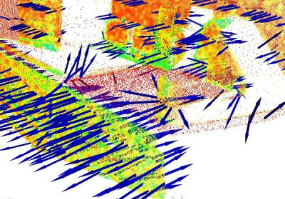
\includegraphics[width=\linewidth]{normales_mal}
  \caption{Vectores normales en una nube de puntos orientados de forma inconsistente.}\label{fig:normales_mal}
\endminipage\hfill
\minipage{0.48\textwidth}
  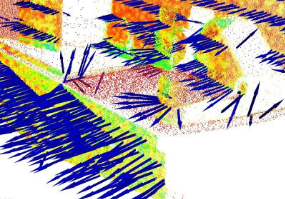
\includegraphics[width=\linewidth]{normales_bien}
  \caption{Vectores normales en una nube de puntos orientados de forma consistente.}\label{fig:normales_bien}
\endminipage\hfill
\end{figure}


\section{Estimación de normales a la superficie de una nube: alto nivel}
Conociendo el fundamento teórico relacionado con la estimación de normales a una superficie representada por un conjunto de puntos, se procede a continuación a explicar cómo PCL implementa este proceso.

Se retoma brevemente el código que permite calcular las normales en una nube de puntos:

\begin{lstlisting}[language=C++,breaklines]
  pcl::PointCloud<pcl::PointNormal>::Ptr cloud_normals (new 		pcl::PointCloud<pcl::PointNormal>);
  pcl::search::KdTree<pcl::PointXYZ>::Ptr tree_n(new pcl::search::KdTree<pcl::PointXYZ>());

  ne.setInputCloud(cloud_xyz);
  ne.setSearchMethod(tree_n);
  ne.setRadiusSearch(radius_search);
 
  std::cout << "Estimating normals in " << filename << " surface..." <<std::endl;

  begin = clock();
  ne.compute(*cloud_normals);
  end = clock();

  normal_estimation_time = double(end-begin)/CLOCKS_PER_SEC;
  std::cout << "Time needed for normal estimation (compute) in " << filename << ": " << normal_estimation_time << " seconds" << std::endl << std::endl;
\end{lstlisting}

Se recuerda que el método que lleva a cabo el algoritmo de estimación es $compute$ y cuyo contenido, explicado en alto nivel, es el que muestra el flujograma de la figura \ref{fig:compute_alto_nivel_diagram}.

\begin{figure}[!htb]
\centering
\minipage{0.5\textwidth}
  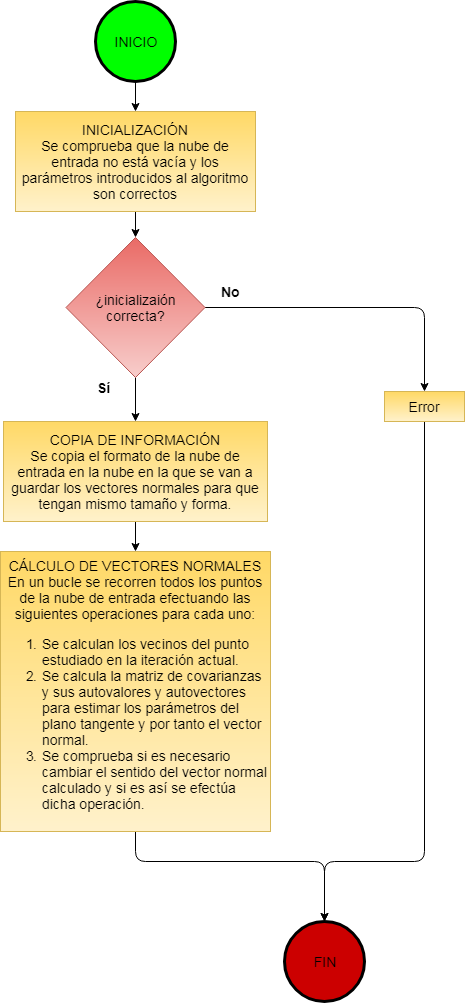
\includegraphics[width=\linewidth]{compute_alto_nivel_diagram}
  \caption{Proceso simplificado de estimación de normales en una nube de puntos.}\label{fig:compute_alto_nivel_diagram}
\endminipage\hfill

\end{figure}

\section{Estimación de normales a la superficie de una nube: bajo nivel}
\subsection{Consideraciones previas}
Para la explicación en bajo nivel (código en C++) de cómo PCL extrae las normales de una nube de puntos, se va a proceder de una forma mixta entre las explicaciones previas en alto y bajo nivel: se plantearán los flujogramas pertinentes cuyo contenido es la parte más relevante del código junto a las aclaraciones necesarias. Se procede de esta forma porque la estimación de normales no queda enteramente contenida al método $compute$ mencionado previamente, es decir, se hacen llamadas a otros métodos de la librería PCL o incluso de librerías externas y las cuales no se explicarán puesto que no son objetivo de optimización.

Para llevar a cabo la explicación, se van a mostrar diferentes flujogramas conectados entre sí, cada uno con una funcionalidad y propósito propios, pero que en conjunto permiten reproducir el algoritmo de estimación de normales en una nube de puntos. Estos flujogramas se dividen en tres tipos: A, B y C que dividen la explicación en proceso de inicialización del algoritmo, estimación de normales y proceso de cierre del algoritmo, respectivamente.

Antes de proseguir con la explicación, se muestra en la figura \ref{fig:compute_esquema_clases} el esquema de los flujogramas que se usarán para la explicación y qué tipo de bloques cabe esperar de cada uno. Además, se indica las clases de PCL utilizadas y la relación de herencia entre ellas. Cabe destacar que:

\begin{itemize}
\item[•]\textit{PCLBase} implementa los métodos utilizados por la mayoría de los algoritmos de toda la librería.
\item[•]\textit{Feature} implementa métodos de estimación de características locales en una nube de puntos, como se ha explicado con anterioridad.
\item[•]\textit{NormalEstimation} implementa métodos específicos de estimación de normales.
\end{itemize} 

Además, en los flujogramas, las partes del código en las que se centra la explicación está resaltada en color rojo.

\begin{figure}[h!]
\centering
\includegraphics[scale=0.4]{compute_esquema_clases}
\caption{Esquema de bloques del flujograma para explicación en bajo nivel y relación entre las clases utilizadas de la librería PCL. En la figura, el flujograma principal se sitúa a la izquierda y hace una llamada a un flujograma A que se desarrolla en la parte derecha.}\label{fig:compute_esquema_clases}
\end{figure}

\subsection{Cuerpo principal del algoritmo}
En la figura \ref{fig:compute_main} se puede ver el cuerpo del algoritmo de extracción de normales. El cuadro con un color naranja más intenso que los demás indica la llamada al método que desencadena todas las operaciones directamente relacionadas con la estimación de normales a parte de los procesos de inicialización y comprobaciones que efectúan los demás bloques. Tanto el desarrollo de la estimación de normales como los procesos auxiliares se implementan en flujogramas separados.

\begin{figure}[h!]
\centering
\includegraphics[scale=0.45]{compute_main}
\caption{Flujograma que representa el cuerpo del algoritmo de estimación de normales. Tiene conexión con otros tres flujogramas etiquetados como A, B y C.}\label{fig:compute_main}
\end{figure}

\subsubsection{Flujogramas tipo A: proceso de inicialización}
Este tipo de flujogramas se refieren al proceso de inicialización explicado en la figura \ref{fig:compute_main}. Este proceso está implementado en la librería de PCL pero no se explica ya que no es de interés para su optimización puesto que implementa operaciones triviales y simples tales como asignaciones y comprobaciones que ocupan una pequeña parte del código.


%\begin{figure}[h!]
%\centering
%\includegraphics[scale=0.5]{compute_init}
%\caption{Flujogramas tipo A que indican el proceso de %inicialización del algoritmo de estimación de normales.}\label{fig:compute_init}
%\end{figure}


\subsubsection{Flujogramas tipo B: estimación de normales}

La figura \ref{fig:compute_compute_feature} muestra el flujograma principal de tipo B que explica el bucle que recorre todos los puntos de la nube y dentro del cual se llaman a tres métodos: $searchForNeighbors$, $computePointNormal$ y $flipNormalTowardsViewpoint$. Estos métodos se explican en sus respectivos flujogramas.

\begin{figure}[h!]
\centering
\includegraphics[scale=0.5]{compute_compute_feature}
\caption{Flujograma tipo B que agrupa la llamada a los métodos necesarios para la estimación de normales}\label{fig:compute_compute_feature}
\end{figure}

Las tres extensiones del flujograma B son B.1, B.2 y B.3 y explican, respectivamente, la búsqueda de vecinos entorno al punto estudiado, el cálculo de la normal en el punto estudiado y el proceso de cambiar de sentido la normal, si fuera necesario. No se muestran en detalle B.1 ni B.3 pues su contenido no está la librería de PCL para el caso del cálculo de vecinos y la operación de voltear un vector es bastante escueta y difícilmente optimizable. Por otra parte, se tiene el corazón del algoritmo en el flujograma B.2 que implementa el método \textit{computePointNormal} en la figura \ref{fig:compute_computePointNormal}) y es el que llama a los métodos que explican el cálculo de la matriz de covarianzas (\textit{computeMeanAndCovarianceMatrix}) y la obtención del vector normal (\textit{solvePlaneParameters}) procesos que se explican en los flujogramas B.2.1 y B.2.2 respectivamente (figuras \ref{fig:compute_computeMean} y \ref{fig:compute_solvePlane})



%\begin{figure}[h!]
%\centering
%\includegraphics[scale=0.5]{compute_neighbors_flip}
%\caption{Flujogramas B.1 y B.3 para la estimación de vecinos y cambiar el sentido al vector normal}\label{fig:compute_neighbors_flip}
%\end{figure}


\begin{figure}[h!]
\centering
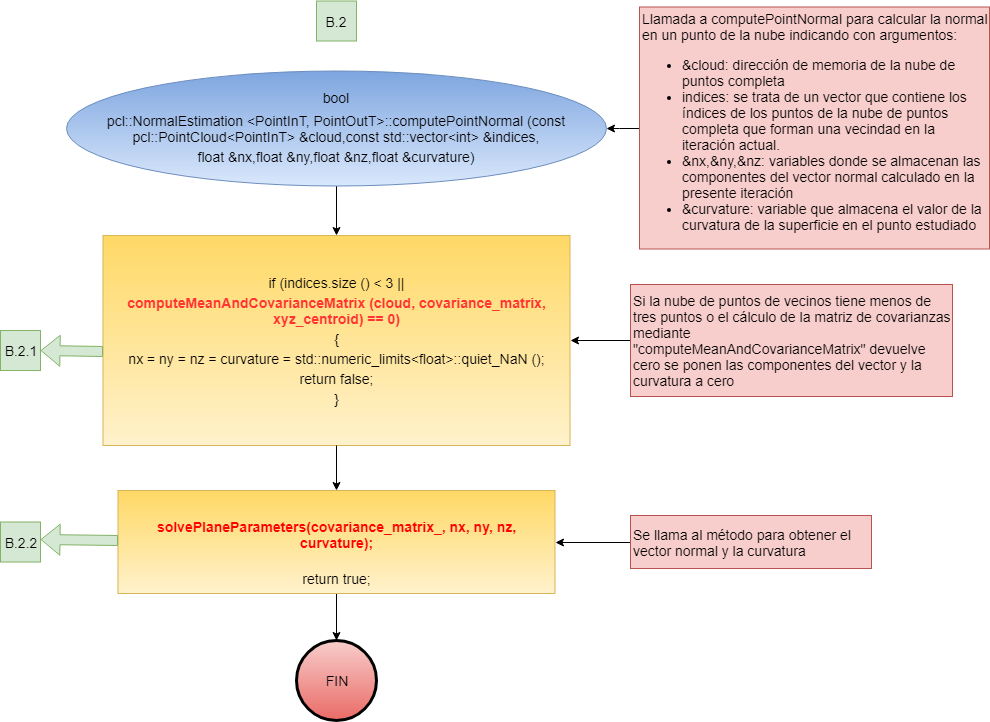
\includegraphics[scale=0.5]{compute_computePointNormal}
\caption{Flujograma B.2 que implementa la estimación de vectores normales.}\label{fig:compute_computePointNormal}
\end{figure}


\begin{figure}[h!]
\centering
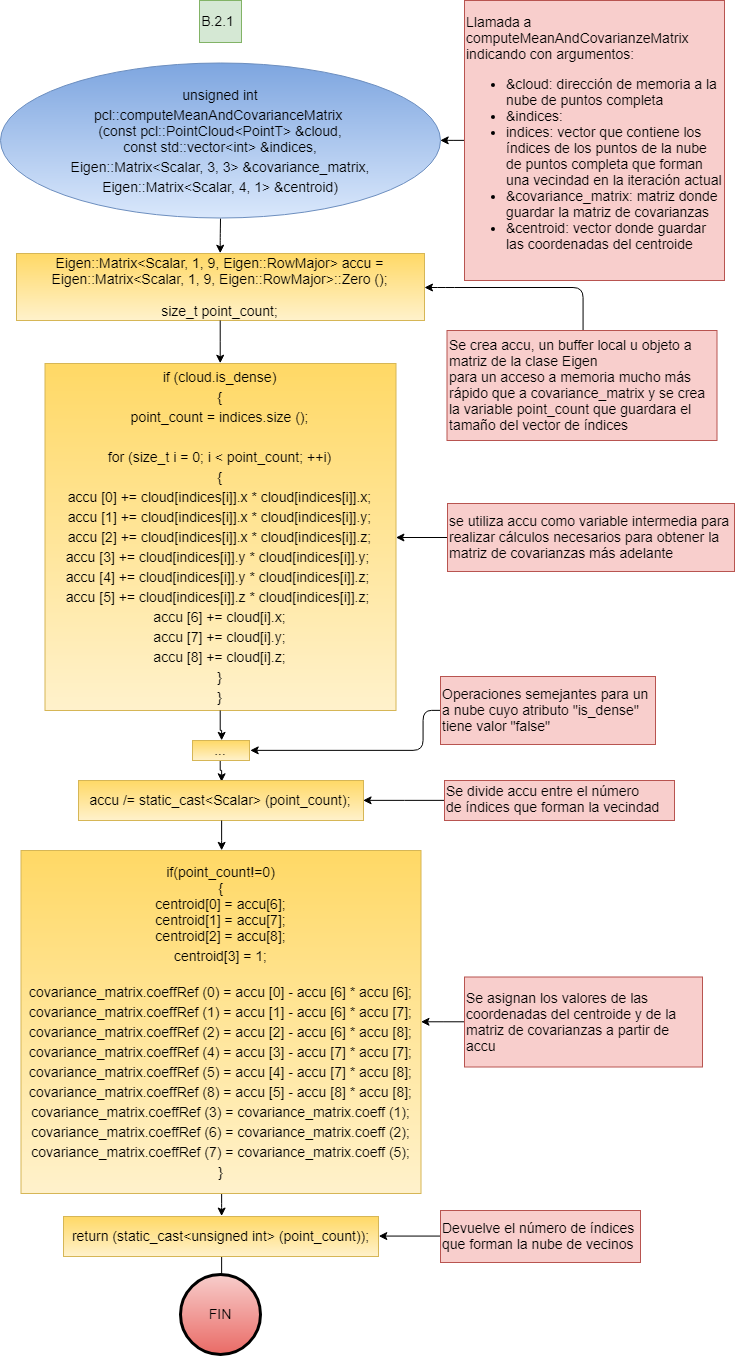
\includegraphics[scale=0.5]{compute_computeMean}
\caption{Flujograma B.2.1 que explica el cálculo de la matriz de covarianzas.}\label{fig:compute_computeMean}
\end{figure}


\begin{figure}[h!]
\centering
\includegraphics[scale=0.5]{compute_solvePlane}
\caption{Flujograma B.2.2 que explica el cálculo de autovalores y autovectores para obtener el vector normal.}\label{fig:compute_solvePlane}
\end{figure}



\subsubsection{Flujogramas tipo C: cierre del algoritmo}
Por último, se tiene un proceso de cierre del algoritmo que enlaza con la comprobación de la superficie de la nube sobre la que se van a buscar normales y que es realizada en la parte de inicialización. No se dan más detalles sobre este proceso ya que es realizado en software y no es objetivo de optimización.


%\begin{figure}[h!]
%\centering
%\includegraphics[scale=0.6]{compute_deinit}
%\caption{Flujograma C que explica la última operación antes del %cierre del algoritmo.}\label{fig:compute_deinit}
%\end{figure}

\section{Selección del fragmento del algoritmo para su optimización}
Se ha mencionado previamente que el núcleo del algoritmo la estimación de vectores normales a la superficie lo conforman el cálculo de matrices de covarianzas y las componentes de cada vector normal.

Se ha decidido seleccionar el cálculo de la matriz de covarianzas explicado en la figura \ref{fig:compute_computeMean} para su optimización puesto que se reduce a operaciones con vectores y matrices que no requieren el uso de librerías específicas a diferencia del cálculo de las componentes del vector normal que necesita utilizar Eigen y da lugar a elementos no sintetizables en hardware. 

\section{Conclusiones}

Se ha explicado en este capítulo tanto a nivel teórico como práctico, es decir, haciendo uso de la librería PCL, la obtención de vectores normales a una superficie definida por una nube de puntos.

En el siguiente capítulo, se mostrarán las modificaciones pertinentes al algoritmo de estimación de normales para que sea sintetizable en hardware y se explicará el proceso de optimización llevado a cabo.
